\documentclass[tikz]{standalone}
\usepackage{tkz-euclide}
\begin{document}
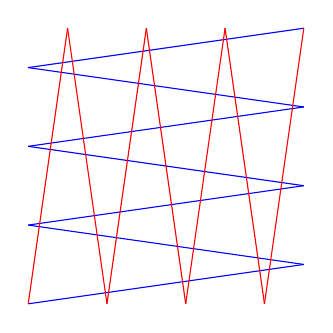
\begin{tikzpicture}[scale=0.5]
	%\tkzInit[xmax=13,ymax=8,xmin=-1,ymin=-1]
	
	\tkzDefPoint(0,0){p1}
	\tkzDefPoint(7,1){p2}
	\tkzDefPoint(0,2){p3}
	\tkzDefPoint(7,3){p4}
	\tkzDefPoint(0,4){p5}
	\tkzDefPoint(7,5){p6}
	\tkzDefPoint(0,6){p7}
	\tkzDefPoint(7,7){p8}

	\tkzDefPoint(0,0){q1}
	\tkzDefPoint(1,7){q2}
	\tkzDefPoint(2,0){q3}
	\tkzDefPoint(3,7){q4}
	\tkzDefPoint(4,0){q5}
	\tkzDefPoint(5,7){q6}
	\tkzDefPoint(6,0){q7}
	\tkzDefPoint(7,7){q8}

	\path[-,color=blue] (p1) edge (p2);
	\path[-,color=blue] (p2) edge (p3);
	\path[-,color=blue] (p3) edge (p4);
	\path[-,color=blue] (p4) edge (p5);
	\path[-,color=blue] (p5) edge (p6);
	\path[-,color=blue] (p6) edge (p7);
	\path[-,color=blue] (p7) edge (p8);

	\path[-,color=red] (q1) edge (q2);
	\path[-,color=red] (q2) edge (q3);
	\path[-,color=red] (q3) edge (q4);
	\path[-,color=red] (q4) edge (q5);
	\path[-,color=red] (q5) edge (q6);
	\path[-,color=red] (q6) edge (q7);
	\path[-,color=red] (q7) edge (q8);
\end{tikzpicture}
\end{document}
